%tex
%% $Id: arbeit.tex 78 2009-07-30 19:49:33Z miracle $
% Bitte verwenden Sie pdflatex.
% Bitte beachten: es mu"s hier eine Sprachangabe gemacht werden.
% Verwenden Sie im Zweifelsfall ngerman.
\documentclass[IN,ngerman,utf8,12pt]{tumbook}
% Optionen f"ur tumbook:

%  Fakult"aten:
%   NEUTRAL -- ohne Logo und Bezeichnung
%   AR   Architektur            BV   Bauingenieur- und Vermessungswesen
%   CH   Chemie                 EI   Elektro- und Informationstechnik
%   IN   Informatik             MA   Mathematik
%   MED  Medizin                MW   Maschinenwesen
%   PH   Physik                 SE   TUM School of Education
%   SP   Sportwissenschaft      WI   Wirtschaftswissenschaften
%   WZW  Wissenschaftszentrum Weihenstephan

%   Sprachen (f"ur Silbentrennung): ngerman, english (siehe babel)
%   Schriftgr"o"sen: 9pt, 10pt, 12pt

\newcommand\todo[1]{\textcolor{red}{TODO: #1}}

\newcommand{\zB}{z.\,B.\ }
\newcommand{\ua}{u.\,a.\ }
\newcommand{\dah}{d.\,h.\ }
\newcommand{\vgl}{vgl.\ }
\newcommand{\oae}{o.\,ä.\ }
\newcommand{\vlt}{vlt.\ }
\newcommand{\bzw}{bzw.\ }
\newcommand{\ggf}{ggf.\ }

\makeindex

% Die klein geschriebenen \title, \author und \date sind obligatorisch.
\Seminar{ETI-Großpraktikum}
\Semester{SS 2013}
\title{Entwicklung eines Logic Analyzers in VHDL}
\Untertitel{ETI-GP 03}
\Themensteller{Georg Acher}
\TUMAdresse{Boltzmannstraße 3, 85748 Garching}
%\Autorenadresse{Anschrift und Telefonnummer des Autors}
%\Matrikelnummer{Matrikelnr. ggf. mit \, gruppiert}
%\Fachsemester{Anzahl der Fachsemester des Autors}
\Abgabetermin{10. August 2013}
\author{Sven Hertle, Markus Engel, Thomas Czok}
%\date{Ort und Datum (f\"ur ehrenw\"ortliche Erkl\"arung)}

\begin{document}
\maketitle%                  Erzeugt die Titelseite
\tableofcontents%            Erzeugt das Inhaltsverzeichnis
\clearpage

\chapter{Was ist ein Logikanalyzer?}
Mit einem Logikanalyzer kann der zeitliche Verlauf von digitalen Signalen aufgenommen werden.
Ein Logikanalyzer zeigt also nur die Werte 0 und 1 an.
Einige Geräte können aber \zB auch noch anzeigen, wenn der aufgenommene Wert undefiniert ist.
Im Gegensatz zu einem Oszilloskop hat ein Logikanalyzer aber eine große Zahl an Eingängen.
Es sind auch Geräte mit mehreren hundert Eingängen verfügbar.
Logikanalyzer werden zum Debuggen von digitalen Schaltungen benötigt.
Dazu benötigt man aber einen großen Speicher oder sehr gute Trigger, da man kaum periodische Vorgänge untersuchen will.

Inzwischen werden Logikanalyzer oft durch Simulationen ersetzt.
Diese können einen Logikanalyzer aber nicht komplett ersetzen.
Auch gegenüber den Diagnoseschnittstellen, die oft in integrierten Schaltkreisen vorhanden sind, hat ein Logikanalyzer Vorteile: Dieser ist oft schneller und genauer.

\chapter{Verwendete Hardware}
Der Logikanalyzer wurde mit dem FPGA-Board GOP\_XC3S200 realisiert.
Dieses ist ausgestattet mit einem Xilinx Spartan 3 XC3S200, der mit 49.152 MHz getaktet wird.
Außerdem befinden sich auf dem Board zwei Taster und acht ansteuerbare LEDs.
Diese wurden aber nicht verwendet, da noch weitere sieben Taster an das Board angeschlossen sind.
Das FPGA-Board ist mit zwei Stiftleisten direkt in einer Steckplatine angebracht.
Darüber sind die weiteren Ein- und Ausgänge sowie die Stromversorgung angeschlossen.

Die aufgezeichneten Daten können über VGA an einem Bildschirm angeschaut werden.
Für den VGA Ausgang werden die Signale HSYNC, VSYNC sowie analoge Werte für die Farben rot, grün und blau benötigt.
Für diese analogen Werte werden jeweils zwei digitale Ausgänge über passende Widerstände zusammengeführt.
Dadurch können 64 verschiedene Farben dargestellt werden.

Der Dateneingang ist 8 Bit breit, es können also acht Kanäle aufgezeichnet werden.
Dazu befindet sich auf der Steckplatine ein Zählbaustein, der durch einen Quarzoszillator mit 50 MHz \todo{sicher? ich dachte es wären etwa 25 Mhz} Taktfrequenz hochgezählt wird.
Dieser dient dem Logikanalyzer als beispielhafte Signalquelle.
Die acht Signale sind mit dem FPGA über die Pins \todo{x bis y} verbunden.

\begin{figure}
    \centerline{
        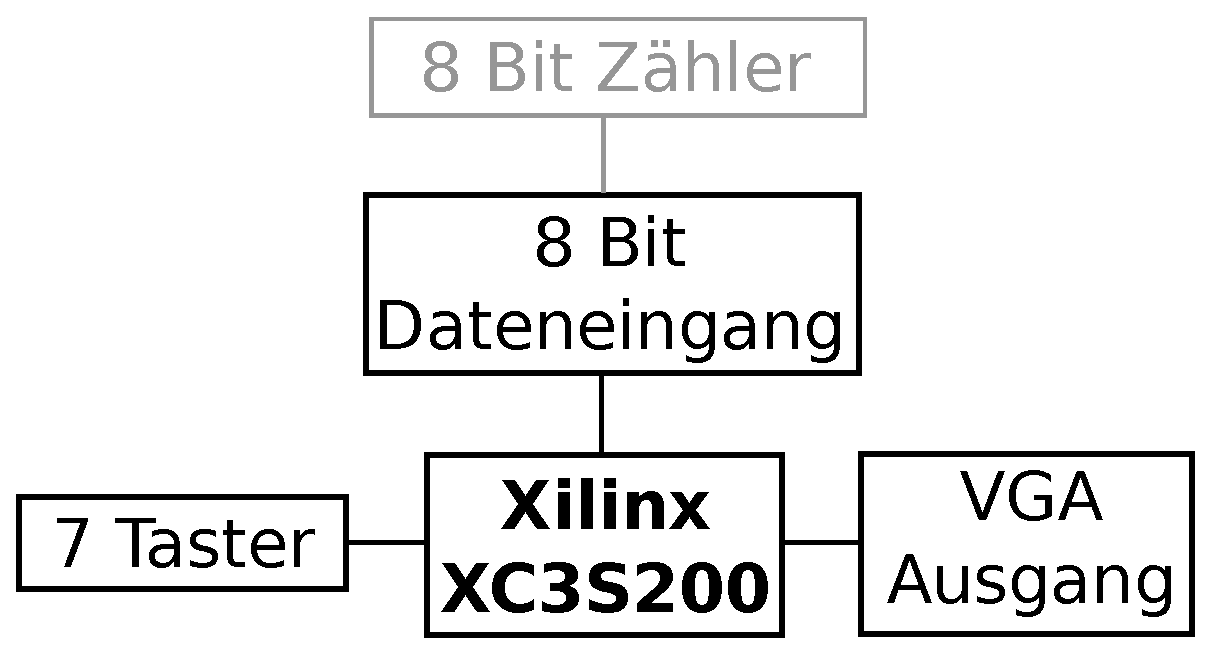
\includegraphics[width=0.5\textwidth]{img/hardware}
    }
    \caption{Schematische Darstellung der Hardware}
\end{figure}

\chapter{Spezifikation der Funktionen}

Unser Logikanalyzer kann acht Kanäle aufzeichnen.
Die Steuerung geschieht über die sieben Taster.
Die VGA Ausgabe erzeugt ein 640x480 Pixel Bild bei 60 Hz.

Es gibt grundsätzlich zwei Aufzeichnungsarten:

\begin{description}
    \item[Continuous] Der Speicher wird als Ring verwendet, \dah die Messdaten werden ständig wieder überschrieben.
        Sobald der Speicher voll wäre, wird vorne wieder angefangen zu schreiben.
    \item[One Shot] Hier wird der Speicher einmal vollgeschrieben, danach stoppt die Aufzeichnung.
        Es passen insgesamt 24.576 Messwerte in den Speicher.
        Dies ist für die Analyse der Signale meist sinnvoller.
\end{description}

Dazu können verschiedene Samplingraten gewählt werden, \dah der Abstand zwischen zwei Aufnahmen.
Dabei sind folgende Werte möglich:

\begin{itemize}
    \item Maximum (20 ns)
    \item 1 ms
    \item 10 ms
    \item 100 ms
    \item 1 s
\end{itemize}

Nach der Aufnahme können die Daten genauer betrachtet werden.
Dazu ist Scrollen und Zoomen möglich.
Dabei wird selbstverständlich eine Zeitskala und der zeitliche Abstand (Timebase) zwischen zwei Strichen angezeigt.
Zum Überfliegen der Messdaten steht schnelles Zoomen zur Verfügung, zum Ausrichten an den Zeitmarkierungen kann dann auch langsam gescrollt werden.
Beim Zoomen entspricht 100\% einem Messwert pro Pixel.
Es sind die Zoomstufen 25\%, 50\%, 100\%, 200\% und 400\% möglich.
Die Timebase wird für jede Zoomstufe und Samplingrate korrekt angezeigt.

Der Logikanalyzer ist auch mit einfachen Triggern ausgestattet.
Pro Kanal kann als Bedingung gewählt werden, dass eine logische 1, 0, eine steigende oder fallende Flanke anliegen soll.
Wenn alle Bedingungen wahr sind, startet die Aufzeichnung.

%Aufgrund der zur Verfügung stehenden Hardware-Ressourcen mussten wir diverse Einschränkungen bei der Festlegung der gewünschten Funktionen unseres Logic Analyzers vornehmen.
%
%\section{Bildspeicher}
%Durch den geringen vorhandenen Block-RAM war es uns nicht möglich, einen kompletten Bildspeicher zu implementieren. Stattdessen sind wir darauf ausgewichen, die Bildsignale direkt aus einem Prozess heraus an den VGA-Ausgang zu senden.
%
%\section{Anzahl der aufnehmbaren Samples}
%Die Anzahl der speicherbaren Messwerte wird ebenfalls ausschließlich durch den RAM beschränkt. ...
%
%\section{Positionierung von Schriftzeichen}
%Da auch die einzelnen Zeichen in einem RAM gehalten werden müssen, haben wir keine freie Positionierung vorgesehen, sondern uns darauf beschränkt, den Bildschirm in 8x8 Pixel große Quadrate (Größe eines Zeichens) zu unterteilen und jedem Quadrat ein Zeichen zuweisen zu können.
%
%\section{Maximale Samplingrate}
%Die maximale einstellbare Samplingrate hängt vom zur Verfügung stehenden Takt ab. Dieser beträgt 49,xy MHz; das entspricht der höchsten Samplingrate.

\chapter{Bedienungsanleitung für Anwender}
Wie benutzt man das Teil? Screenshots mit Erklärung?

\chapter{Dokumentation für Entwickler}

Der Logikanalyzer wurde mit VHDL implementiert.
Dazu wurde die Software Xilinx ISE WebPACK verwendet.

\section{Komponenten}

Der Logikanalyzer ist in verschiedene Komponenten unterteilt.
Diese werden in Abb. \ref{abb:komp} dargestellt.

\begin{figure}
    \centerline{
        \includegraphics[width=0.5\textwidth]{img/komponenten}
    }
    \label{abb:komp}
    \caption{Unterteilung des Logikanalyzers in Komponenten}
\end{figure}

\subsection{Logikanalyzer}
\todo{Diagramme für Blackbox Sicht -> Ein-/Ausgänge erklären}

Die Komponente Logikanalyzer übernimmt die Steuerung aller anderen Komponenten.
Sie beinhaltet alle Signale, die den Status der Logikanalyzers speichern.
Die zur Steuerung verwendeten Taster werden hier ausgewertet.
Die Signale werden dann entsprechend verändert, sodass die vom Benutzer gewünschte Aktion geschieht.

\subsection{RAM}

Zum Speichern der Messwerte wird ein Dualport Block RAM verwendet.
Dieser hat den Vorteil, dass gleichzeitig Daten gelesen und geschrieben werden können.
Dies ist nötig, da ja gleichzeitig Messwerte aufgenommen und Daten auf dem Bildschirm angezeigt werden sollen.
Der RAM wurde mit dem Core Generator aus Xilinx ISE generiert.
Für Änderungen ist daher mindestens Xilinx ISE Version \todo{Markus, welche Version?} nötig.

\subsection{Sampler}

Der Sampler hat die Aufgabe, die Messwerte im RAM zu speichern.
Dabei muss die gewählte Samplingrate sowie der Aufnahmemodus beachtet werden.
Außerdem müssen die aktuell an den Eingängen anliegenden Messwerte an den Sampler weitergegeben werden.
Dieser braucht die aktuellen Daten, um zu entscheiden, ob die Aufnahme gestartet werden soll.

\subsection{Trigger}

Der Trigger entscheidet, ob die Aufnahme gestartet werden soll.
Grundlage dafür sind die Einstellungen des Benutzers und die aktuellen Messwerte.

\subsection{VGA}

Die Komponente VGA erzeugt ein VGA Signal mit 640x480 Pixel und 60 Hz.
Diese Größe und Frequenz wurde gewählt, da der Pixeltakt dann bei 25 MHz liegt, was grob dem halbem Takt des Bausteins (49.152 MHz) entspricht.
Die Abweichung ist klein genug, sodass sie keine Rolle spielt.

Diese Komponente bekommt als Eingabe alle Informationen über das darzustellende Bild:

\todo{Liste}

Dementsprechend wird die Ausgabe dann gezeichnet.
Da nicht genug Speicher für einen Bildspeicher verfügbar ist, wird in jedem Takt entschieden, welche Farbe der aktuelle Pixel hat.
Dazu muss man für jeden Pixel, an den etwas gezeichnet werden soll, abfragen, ob dieser aktuell gezeichnet wird.
Wenn dies der Fall ist, muss die passende Farbe auf die VGA Ausgänge gelegt werden.
Es wurden Prozeduren geschrieben, die das Zeichnen von Linien, Rechtecken und Texten übernehmen.

Damit das Zeichnen der Texte nicht zu aufwändig wird, wird dafür ein Bildspeicher verwendet:
Die einzelnen Zeichen sind 8x8 Pixel groß und können nur in einem Raster mit 8 Pixel Abstand angeordnet werden.
So können insgesamt 80x60 Zeichen dargestellt werden.
Diese werden in einem Array gespeichert, was einem Bildspeicher entspricht.
Da hier aber nur die ASCII Werte der Zeichen gespeichert werden, verbraucht dies nicht zu viel Speicherplatz.
Man muss darauf achten, dass alle Strings gleich lang sind, wenn man an eine Stelle abwechselnd unterschiedliche Texte schreiben will.
Die Prozedur \texttt{drawString} schreibt den Text in den Bildspeicher.
Wenn dieser zu kurz ist, bleibt noch das Ende der vorherigen Textes übrig.
Hier muss man also noch mit Leerzeichen auffüllen.

Beim Zeichnen der aufgezeichneten Signale werden noch steigende und fallende Flanken ergänzt.
Dabei wird einfach bei einem Wechsel des Signals eine senkrechte Linie dazu gezeichnet.

\subsection{TextROM}

Der TextROM ist nur ein Speicher für die Schriftzeichen.
Dabei wird für einen ASCII Wert das Zeichen als 8x8 Pixel Grafik gespeichert.
Die Tabelle enthält aktuell nur Großbuchstaben, Zahlen und einige Sonderzeichen, um Platz zu sparen.
Die Schriftzeichen wurden aus dem Linux Kernel übernommen.

\chapter{Schlusswort}
Was haben wir gelernt? Hats uns Spaß gemacht?

%\nocite{*}% Dieser Befehl bewirkt, dass alle in der Bibliographie-Datei
% aufgef"uhrten Werke auch ausgegeben werden. Sonst werden nur diejenigen
% ausgegeben, die auch zitiert werden.

\clearpage
\appendix%                   Einleitung der Anh"ange
% Die Angabe von \listoftables, index etc. funktioniert,
% wurde aber nicht ausdr"ucklich fuer die TUM angepa"st.
\listoffigures%              Abbildungsverzeichnis
%\bibliographystyle{tumbib} % TUM-spezifische Darstellung der Bibliographie
%\bibliography{arbeit}%       Name der .bib Datei mit der bibliographischen DB
%\clearpage
%\Ehrenwort%                  Ehrenw"ortliche Erkl"arung
\end{document}
